\documentclass[
    NAME={Dr. Helga Ingimundardóttir},
    EMAIL={helgaingim@hi.is},
    FACULTY={Industrial Engineering},
    TITLE={Using Pull Requests to Make Collaboration Visible in CDIO Project-Based Courses},
    SEMINAR={22\textsuperscript{nd} International CDIO Conference},
    DATE={June 22\textsuperscript{nd} 2026},
    WIDE=true
]{HI-LaTeX/hi-beamer}
\setbeameroption{show notes on second screen}
\usepackage{tikz}
\usetikzlibrary{fit,matrix,backgrounds}
\usetikzlibrary{arrows.meta,positioning}

\usepackage[fixed,style=solid]{fontawesome7}

\begin{document}

%------------------------------------------------
\begin{frame}{Motivation}
\begin{block}{\faBuildingColumns~Project-based courses}
Assessment often prioritizes final artifacts, limiting visibility into collaboration, reasoning, and responsiveness to feedback
\end{block}

\begin{block}{\faGithub~Professional practice}
Modern technical work relies on version control, peer review, and documented iteration--skills students are expected to use immediately in the workforce
\end{block}

\begin{alertblock}{\faScaleBalanced~Assessment misalignment}
What we value in learning is not always what we can currently observe
\end{alertblock}
\end{frame}
\note{
Project-based courses are widely used -- and we care about \emph{collaboration}, \emph{reasoning}, and \emph{responsiveness to feedback}.  

But in practice, assessment still prioritizes \emph{final artifacts} -- reports, code, presentations.  

At the same time, professional work is inherently \emph{collaborative} and \emph{iterative}.  

Version control, peer review, and documented iteration are not optional -- they are core practice.  

So the tension is this -- what we value in learning is not always what we can actually \emph{observe and assess}.
}
%------------------------------------------------
\begin{frame}{Framing the problem}
\begin{exampleblock}{\faDumbbell~Core question}
How can collaboration, accountability, and responsiveness to feedback be made \emph{visible and assessable} in team-based projects?
\end{exampleblock}
\begin{itemize}
    \item final deliverables hide process and contribution
    \item peer interaction is difficult to audit retrospectively
    \item feedback often resets instead of accumulating
\end{itemize}
\end{frame}
\note{
This leads to the core question --  

How do we make \emph{collaboration}, \emph{accountability}, and \emph{responsiveness to feedback} visible and assessable?  

In team projects, the final deliverable hides most of what matters -- who did what, how decisions were made, and how feedback was handled.  

Peer interaction is difficult to reconstruct after the fact -- and feedback often \emph{resets} instead of accumulating.  

So the issue is not lack of activity -- it is lack of \emph{visibility}.
}
%------------------------------------------------
\begin{frame}{Learning with professional collaboration tools}
\begin{exampleblock}{\faToolbox~Not just another tool}
Git/GitHub is an industry-standard collaboration infrastructure
\end{exampleblock}
\begin{itemize}
    \item used across software, data science, and engineering teams
    \item supports version control, review, and reproducible handover
    \item directly transferable -- students can credibly list this on their CV
\end{itemize}

\vspace{.5em}

\emph{\faFaceGrinStars\ Motivation: students practice skills they will immediately use}

\end{frame}

\note{
The approach is to use professional collaboration tools -- not as an add-on, but as part of the learning environment.  

Git and GitHub are widely used across technical fields.  

They support \emph{version control}, \emph{peer review}, and \emph{reproducibility}.  

Importantly, these are skills students are expected to use immediately after graduation.  

So this is not just about authenticity -- it is about \emph{transfer}.  
Students practice what they will actually use.
}
%------------------------------------------------
\begin{frame}{Minimal GitHub concepts (for assessment)}
\begin{block}{\faDatabase~Repository}
A shared workspace containing code, data, documentation, and history
\end{block}

\begin{block}{\faCodePullRequest~Pull Request (PR)}
A structured proposal to change shared work, including:
\begin{itemize}
    \item rationale and scope
    \item peer review and discussion
    \item explicit approval and merge decision
\end{itemize}
\end{block}

\emph{\faKey\ Key idea: PRs bind technical change to collaborative process}

\end{frame}
\note{
Briefly aligning terminology --  

A repository is a shared workspace containing code, data, and history.  

A pull request -- or PR -- is a structured proposal to change shared work.  

It includes a rationale, and is reviewed, discussed, and approved before merging.  

The key idea is that PRs bind \emph{technical change} to \emph{collaborative process}.
}
%------------------------------------------------
\begin{frame}{Design rationale}
\begin{columns}[T,onlytextwidth]
\begin{column}{.38\textwidth}
\begin{block}{\faCompassDrafting~Starting point}
\begin{itemize}
    \item CDIO-aligned
    \item assessment as development
    \item observable collaborative
\end{itemize}
\end{block}
\end{column}
\begin{column}{.58\textwidth}
\begin{alertblock}{\faKey~Design claim}
Pull requests are not treated as a tooling detail, but as \emph{assessment infrastructure}:
\[
\faComments~\text{feedback}
\;+
\faRepeat~\text{iteration}
\;\Rightarrow\;
\faMedal~\text{competence}
\]
\end{alertblock}
\end{column}
\end{columns}
\end{frame}
\note{
The design is CDIO-aligned and treats assessment as a \emph{developmental process}.  

The focus is on \emph{observable collaboration}, not just outcomes.  

The central claim is that pull requests are not just a tool -- but can function as \emph{assessment infrastructure}.  

They make feedback and iteration visible -- and over time this supports competence development.
}
%------------------------------------------------
\begin{frame}{Why pull requests matter}
\begin{columns}[T,onlytextwidth]
\begin{column}{.44\textwidth}
\begin{block}{\faDatabase~Repository}
A shared workspace containing code, data, documentation, and history
\end{block}
\begin{block}{\faCodePullRequest~Pull Request (PR)}
A structured proposal to change shared work through:
\begin{itemize}
    \item rationale and scope
    \item peer review and discussion
    \item approval and merge decision
\end{itemize}
\end{block}
\end{column}
\begin{column}{.51\textwidth}
\begin{exampleblock}{\faMagnifyingGlass~Why it matters for assessment}
\begin{itemize}
    \item reasoning becomes visible
    \item contribution becomes attributable
    \item critique and negotiation are captured
    \item responses to feedback are auditable
\end{itemize}
\end{exampleblock}
\vspace{0.4em}
\begin{alertblock}{\faLightbulb~Reframing}
PRs expose the learning process
\end{alertblock}
\end{column}
\end{columns}
\end{frame}
\note{
A PR naturally contains what we want to assess --  

rationale, critique, discussion, and decisions.  

This means reasoning becomes \emph{visible},  
contributions become \emph{attributable},  
and responses to feedback become \emph{auditable}.  

So the reframing is simple -- PRs expose the learning process.
}
%------------------------------------------------
\begin{frame}{Assessable behaviors made visible}
\begin{columns}[T,onlytextwidth]
\begin{column}{.48\textwidth}
\begin{block}{\faClipboardList~Required practices}
\begin{itemize}
    \item focused PRs with clear intent
    \item at least two substantive reviews
    \item explicit responses to all comments
    \item merge only after review
\end{itemize}
\end{block}
\end{column}
\begin{column}{.48\textwidth}
\begin{block}{\faUserCheck~Observable evidence}
\begin{itemize}
    \item authorship and co-authorship
    \item depth of critique and follow-up
    \begin{itemize}
        \item[\faGavel] actionable comments (no \texttt{LGTM} or \faThumbsUp)
    \end{itemize}
    \item handover quality
    \item documentation updates
\end{itemize}
\end{block}
\end{column}
\end{columns}
\centering\resizebox{.8\linewidth}{!}{\begin{figure}[b]
\centering
\begin{tikzpicture}[
    x=1cm, y=1cm,
    seg/.style={line width=0.5pt},
    prseg/.style={line width=2pt},
    prmerge/.style={-{Latex[length=2.2mm]}, line width=2pt},
    sync/.style={-{Latex[length=2mm]}, dashed, line width=1.0pt},
    commit/.style={circle, draw, fill=black, inner sep=1.7pt},
    lbl/.style={font=\small},
    ann/.style={font=\small\itshape}
]

% Lane labels
\node[lbl, anchor=east] at (1.6,3.6) {\texttt{main}: \faUsers~ABC};
\node[lbl, anchor=east] at (1.6,2.8) {\texttt{core-work}: \faUser~A};
\node[lbl, anchor=east] at (1.6,2.0) {\texttt{feat-1}: \faUser~B};
\node[lbl, anchor=east] at (1.6,1.2) {\texttt{feat-2}: \faUser~C};

% Main line
\node[commit] (m0) at (3.0,3.6) {};
\node[commit] (m1) at (8.6,3.6) {};
\node[commit] (m2) at (10.8,3.6) {};
\draw[seg] (m0) -- (m1);
\draw[seg] (m1) -- (m2);

\node[ann, anchor=south] at (m0.north) {template};
\node[ann, anchor=south] at (m2.north) {final result};

% Core-work branch from main
\draw[seg] (m0) .. controls (3.3,3.3) and (3.6,3.0) .. (4.0,2.8);
\node[commit] (a1) at (4.0,2.8) {};
\node[commit] (a2) at (5.0,2.8) {};
\node[commit] (a3) at (6.1,2.8) {};
\node[commit] (a4) at (7.2,2.8) {};
\node[commit] (a5) at (9.0,2.8) {};
\draw[seg] (a1) -- (a2);
\draw[seg] (a2) -- (a3);
\draw[seg] (a3) -- (a4);
\draw[seg] (a4) -- (a5);

% feature-B branches from core-work and returns later to core-work
\draw[seg] (a2) .. controls (5.2,2.5) and (5.4,2.2) .. (5.7,2.0);
\node[commit] (b1) at (5.7,2.0) {};
\node[commit] (b2) at (6.5,2.0) {};
\draw[seg] (b1) -- (b2);

% feature-B merged back into a later point on core-work
\draw[prmerge] (b2) .. controls (7.0,2.15) and (7.1,2.45) .. (a4);

% feature-C branches from same initial node as core-work
\draw[seg] (m0) .. controls (3.2,3.0) and (3.7,1.5) .. (4.3,1.2);
\node[commit] (c1) at (4.3,1.2) {};
\node[commit] (c2) at (6.0,1.2) {};
\node[commit] (c3) at (7.3,1.2) {};
\node[commit] (c4) at (7.9,1.2) {};
\draw[seg] (c1) -- (c2);
\draw[prseg] (c2) -- (c3);
\draw[prseg] (c3) -- (c4);

% feature-C merged to main after an extra commit
\draw[prmerge] (c4) .. controls (8.4,1.9) and (8.5,3.0) .. (m1);

% core-work syncs from main after C merge
\draw[sync] (m1) .. controls (8.7,3.25) and (8.9,3.0) .. (a5);
\node[ann, anchor=west] at (8.7,3.25) {sync};

% core-work merged to final main
\draw[prmerge] (a5) .. controls (9.5,3.05) and (10.0,3.35) .. (m2);

% Right-aligned review annotations
\node[ann, anchor=west] at (11.7,3.6) {feedback: \faChalkboardTeacher};
\node[ann, anchor=west] at (11.7,2.8) {review: \faUser~\textup{B}, \faUser~\textup{C}};
\node[ann, anchor=west] at (11.7,2.0) {review: \faUser~\textup{A}, \faUser~\textup{C}};
\node[ann, anchor=west] at (11.7,1.2) {review: \faUser~\textup{A}, \faUser~\textup{B}};

\end{tikzpicture}
\caption{PR-centered interaction workflow for one IE project cycle. Students work on separate branches and integrate changes through reviewed pull requests. The PR phase is highlighted by thicker edges, indicating reviewed integration rather than independent work. 
}

\label{fig:ie-pr-workflow}
\end{figure}}
\end{frame}
\note{
We define specific required practices.  

Students submit focused PRs, receive at least two \emph{substantive} reviews,  
and respond explicitly to all comments.  

Substantive means actionable feedback -- not just superficial approval  

Assessment then uses observable evidence -- authorship, critique, follow-up, and handover.  

So assessment shifts from hidden process to \emph{visible artifacts}.
}
%------------------------------------------------
\begin{frame}{Scaffolded progression across courses}
\begin{columns}[T,onlytextwidth]
\begin{column}{.48\textwidth}
\begin{block}{\faUser~Information Engineering (IE)}
\begin{itemize}
    \item 20--25 students
    \item 6--7 small teams
    \item early undergraduate
    \item new repository each cycle
\end{itemize}
\begin{block}{\faToolbox~Main purpose}
Tooling and collaboration practices are the learning focus
\end{block}
\end{block}
\end{column}
\begin{column}{.48\textwidth}
\begin{block}{\faUserGraduate~Business Intelligence (BI)}
\begin{itemize}
    \item 10--15 students
    \item 2 large teams
    \item assumes GitHub fluency
    \item single persistent repository
\end{itemize}
\begin{block}{\faLayerGroup~Main purpose}
Tooling supports more advanced project work
\end{block}
\end{block}
\end{column}
\end{columns}
\end{frame}
\note{
This is implemented across two courses.  

In Information Engineering, the focus is learning the tools -- small teams, repeated practice, new repositories.  

In Business Intelligence, students are assumed fluent -- one persistent repository across the semester.  

So there is progression -- from learning the workflow to using it as \emph{infrastructure}.
}
%------------------------------------------------
\begin{frame}{Feedback carry-forward}
\begin{columns}[T,onlytextwidth]
\begin{column}{.56\textwidth}
\begin{block}{\faArrowsRotate~Cumulative assessment}
\begin{itemize}
    \item unresolved PR comments remain active
    \item later work is checked against prior feedback
    \item capstone evaluation includes earlier issues
\end{itemize}
\end{block}
\end{column}
\begin{column}{.40\textwidth}
\begin{exampleblock}{\faBullseye~Effect}
\begin{itemize}
    \item continuity
    \item accountability
    \item coherence
    \item less fragmentation
\end{itemize}
\end{exampleblock}
\end{column}
\end{columns}
\end{frame}
\note{
When teams are working with a single, persistent repository, feedback can carry forward -- it doesn't reset between assignments.

If an issue is raised in a pull request and not resolved, it remains visible in the repository.  

Later work is then evaluated in light of that earlier feedback -- including in the capstone.  

So feedback accumulates over time rather than fragmenting across tasks.  

This creates \emph{continuity} and \emph{accountability}.  

Students cannot simply move on -- they have to revisit and resolve issues.  

And that is much closer to professional practice.
}
%------------------------------------------------
\begin{frame}{Indicative evidence}
\centering
\resizebox{.90\linewidth}{!}{
\scriptsize
\renewcommand{\arraystretch}{1.5}
\begin{table}[t]
\centering
\footnotesize
\renewcommand{\arraystretch}{1.1}
\caption{Rubric used to assess GitHub collaboration practices in the IE course}\label{tbl:IE-rubric}
\begin{tabular}{c p{4.4cm} p{4.3cm} p{3.5cm} }
\toprule
 & \textbf{Excellent} & \textbf{Good} & \textbf{Insufficient} \\
\midrule

\rotatebox[origin=r]{90}{GitHub usage}
& Branches are well organized with logical names tied to features. Commits are coherent and clearly describe changes. Documentation is complete and provides clear instructions.
& Branches are used but naming or scope is sometimes inconsistent. Commits are mostly coherent with occasional issues. Documentation is present but incomplete.
& Branches are absent or unclear. Commits are inconsistent with little structure. Documentation is unclear or missing.
\\

\addlinespace

\rotatebox[origin=r]{90}{Teamwork}
& All team members actively contribute. Contributions and responsibilities are distributed across the team. Decisions are shared through review and discussion.
& Most members participate, but contributions are uneven. One or two members lead development, while others contribute through reviews or comments.
& Work is largely carried out by one individual. Participation is minimal or uneven across the team.
\\

\bottomrule
\end{tabular}
\end{table}}
\vfill
\begin{columns}[T,onlytextwidth]
\small
\begin{column}{.47\textwidth}
\begin{exampleblock}{\faArrowTrendUp~Calibration}
\begin{itemize}
    \item levels: developmental\faArrowRight outstanding
    \item same dimensions, increasing expectations
    \item signals expectations for Capstone
\end{itemize}
\end{exampleblock}
\end{column}
\begin{column}{.50\textwidth}
\begin{block}{\faChartLine~Observed trend}
\begin{itemize}
    \item GitHub usage improved over repeated cycles
    \item teamwork \& participation improved more strongly
\end{itemize}
\end{block}
\end{column}
\end{columns}
\end{frame}
\note{
To clarify the rubric design --  

The GitHub usage and teamwork dimensions are \emph{shared across both courses}.  
Early on, we are deliberately \emph{lenient} -- students are still learning the workflow.  

We observe improvement in GitHub use and stronger improvement in teamwork and participation.  
Qualitatively, PRs become more focused, better documented, and more responsive.  

In the BI course, each thematic module also has its own rubric --  
and these are \emph{reused directly in the capstone}.  

During the learning phase, grading is \emph{normalized to ``very good''}.  
So students are not penalized for early-stage work --  

but they are explicitly shown what will be expected in a more \emph{refined, final version}.  

This allows them to \emph{prioritize effort} --  
they can revisit earlier work, address feedback, and align with final expectations in the capstone.  

So students are not only evaluated -- they are shown what ``good enough'' looks like \emph{before} the capstone.  
}
%------------------------------------------------
\begin{frame}{Balancing team and individual assessment}
\begin{columns}[T,onlytextwidth]
\begin{column}{.48\textwidth}
\begin{block}{\faUsers~Team-level}
\begin{itemize}
    \item analytical quality
    \item coherence
    \item shared responsibility
\end{itemize}
\end{block}
\end{column}
\begin{column}{.48\textwidth}
\begin{block}{\faUserCheck~Individual-level}
\begin{itemize}
    \item visible contributions
    \item review quality
    \item responsiveness to feedback
\end{itemize}
\end{block}
\end{column}
\end{columns}
\vspace{0.4em}
\begin{alertblock}{\faScaleBalanced~Design goal}
Accountability without fragmenting teamwork
\end{alertblock}
\end{frame}
\note{
A common concern is balancing team and individual assessment.  

Team-level outcomes still matter -- quality and coherence.  

But individual contribution becomes visible through artifacts -- commits, reviews, and discussion.  

The goal is \emph{accountability} without breaking \emph{collaboration}.
}
%------------------------------------------------
\begin{frame}{Key shifts in practice}
\begin{columns}[T,onlytextwidth]
\begin{column}{.30\textwidth}
\begin{block}{\faShieldHalved~Quality}
\centering iteration\\ vs.\ reviewable work
\end{block}
\end{column}
\begin{column}{.30\textwidth}
\begin{block}{\faUsers~Collaboration}
\centering implicit teamwork\\ vs.\ explicit review
\end{block}
\end{column}
\begin{column}{.30\textwidth}
\begin{block}{\faLaptopCode~Workflow}
\centering informal work\\ vs.\ structured process
\end{block}
\end{column}
\end{columns}
\vspace{0.4em}
\begin{alertblock}{\faLightbulb~Takeaway}
Making collaboration visible turns implicit practices into something we can teach and assess
\end{alertblock}
\end{frame}
\note{
What PR-based workflows do is make collaboration practices \emph{explicit}.  

Students are not used to reviewing each other's work critically.  
That's not a problem -- it's something we need to \emph{teach and normalize}.  

Similarly, work becomes visible much earlier.  
Students can no longer rely on polishing something at the end -- they have to produce work that can be reviewed along the way.  

And the workflow itself introduces structure.  
That can feel like overhead, but it is also what enables learning -- especially around collaboration and feedback.  

So rather than thinking of these as problems or tensions,  
they are \emph{practices becoming visible} -- and therefore teachable.
}
%------------------------------------------------
\begin{frame}{Limitations and next steps}
\begin{columns}[T,onlytextwidth]
\begin{column}{.48\textwidth}
\begin{block}{\faLock~Boundary conditions}
\begin{itemize}
    \item design-oriented, not experimental
    \item depends on student readiness
    \item larger cohorts require more coordination
\end{itemize}
\end{block}
\end{column}
\begin{column}{.48\textwidth}
\begin{block}{\faArrowTrendUp~Next iterations}
\begin{itemize}
    \item extend to more courses
    \item structured team-building to accelerate trust
    \item refined review calibration
\end{itemize}
\end{block}
\end{column}
\end{columns}
\end{frame}
\note{
There is definitely some initial overhead -- especially around learning the workflow and review practices.  

Students are not used to this level of structure or visibility.  

It also depends on readiness -- this works much better once basic tooling is already in place.  

And scaling requires coordination, particularly around review quality.  

So this is not a drop-in solution -- it needs to be designed into the course.
}
%------------------------------------------------
\begin{frame}{Conclusions}
\begin{exampleblock}{\faFlagCheckered~Key takeaway}
PR-based assessment makes collaboration, accountability, and responsiveness to feedback visible and assessable
\end{exampleblock}
\begin{itemize}
    \item assessment moves from final products to visible process
    \item feedback carries forward instead of resetting
    \item students practice professional collaboration in routine course work
\end{itemize}
\vspace{0.4em}
\begin{alertblock}{\faLightbulb~Contribution}
This is an assessment architecture, not just a tool choice
\end{alertblock}
\end{frame}
\note{
The key takeaway is that making collaboration visible fundamentally changes what we can assess.  

There is an initial overhead -- students don't always enjoy the structure at first.  
Reviewing peers, documenting work, responding to feedback -- this is unfamiliar and effortful.  

But over time, the quality of work improves significantly.  
Work becomes more structured, better justified, and more coherent.  

And importantly, students recognize this afterwards.  
Many of them explicitly say that this is where they learned the most -- not just the content, but how to actually work.  

So the impact is not just in what they produce --  
it's in how they approach collaboration, feedback, and responsibility.  

And that comes from the \emph{assessment structure}, not the specific subject matter.
}
%------------------------------------------------
\begin{frame}{Questions?}
    \begin{columns}        
        \begin{column}{0.5\textwidth} 
        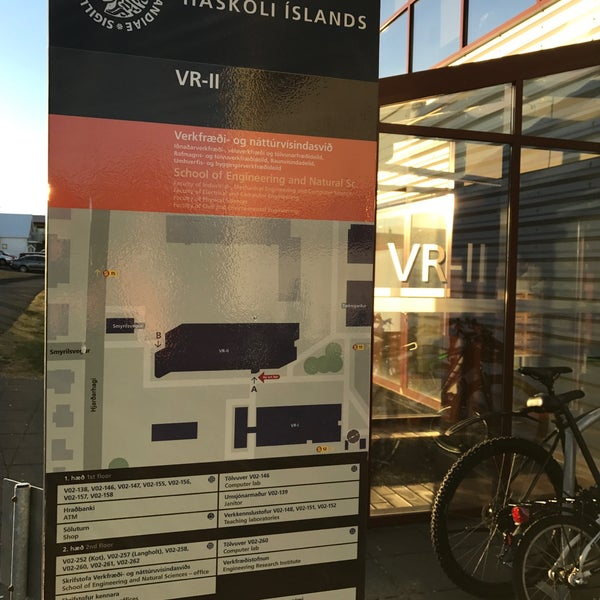
\includegraphics[height=\textwidth]{include/vr2.jpg}
        \end{column}
        \hfill
        \begin{column}{0.4\textwidth}         
            \begin{exampleblock}{Contact details:}            
            \begin{itemize}
                \item[\faEnvelope] helgaingim@hi.is
                \item[\faPhone] +354 525-4630
                \item[\faBuildingColumns] VR-II, University of Iceland
                \item[\faLinkedin] helgaingimundardottir
                \item[\faGithub] @tungufoss
            \end{itemize}
            \end{exampleblock}
            \end{column}
    \end{columns}    
\end{frame}
\note{
A few questions that often come up --  

\emph{Isn't this a lot of overhead?}  
Yes -- there is initial overhead.  
But it decreases quickly, and the payoff is that assessment becomes much easier and more transparent later.  

\emph{What about students with no GitHub experience?}  
We scaffold this earlier in the curriculum.  
In later courses, we assume fluency so the tooling does not dominate the learning.  

\emph{Does this scale?}  
It can scale, but requires coordination -- especially around review practices.  
The visibility actually helps manage larger groups.  

\emph{How do you ensure fairness in team assessment?}  
Individual contributions are visible through PRs, reviews, and discussion.  
So we don't rely only on peer evaluation -- we have \emph{artifact-based evidence}.  

\emph{Is this specific to software or data courses?}  
The tooling is domain-specific, but the principle is not.  
The idea is to make process and feedback visible -- the same logic can apply elsewhere.  

\emph{Is this just about GitHub?}  
No -- GitHub is the \emph{enabler}.  
The contribution is the \emph{assessment architecture}.  
}

\end{document}

